\documentclass[]{article}
\usepackage{lmodern}
\usepackage{amssymb,amsmath}
\usepackage{ifxetex,ifluatex}
\usepackage{fixltx2e} % provides \textsubscript
\ifnum 0\ifxetex 1\fi\ifluatex 1\fi=0 % if pdftex
  \usepackage[T1]{fontenc}
  \usepackage[utf8]{inputenc}
\else % if luatex or xelatex
  \ifxetex
    \usepackage{mathspec}
  \else
    \usepackage{fontspec}
  \fi
  \defaultfontfeatures{Ligatures=TeX,Scale=MatchLowercase}
\fi
% use upquote if available, for straight quotes in verbatim environments
\IfFileExists{upquote.sty}{\usepackage{upquote}}{}
% use microtype if available
\IfFileExists{microtype.sty}{%
\usepackage{microtype}
\UseMicrotypeSet[protrusion]{basicmath} % disable protrusion for tt fonts
}{}
\usepackage[margin=1in]{geometry}
\usepackage{hyperref}
\hypersetup{unicode=true,
            pdftitle={ABCLakrids},
            pdfauthor={Smilk},
            pdfborder={0 0 0},
            breaklinks=true}
\urlstyle{same}  % don't use monospace font for urls
\usepackage{color}
\usepackage{fancyvrb}
\newcommand{\VerbBar}{|}
\newcommand{\VERB}{\Verb[commandchars=\\\{\}]}
\DefineVerbatimEnvironment{Highlighting}{Verbatim}{commandchars=\\\{\}}
% Add ',fontsize=\small' for more characters per line
\usepackage{framed}
\definecolor{shadecolor}{RGB}{248,248,248}
\newenvironment{Shaded}{\begin{snugshade}}{\end{snugshade}}
\newcommand{\KeywordTok}[1]{\textcolor[rgb]{0.13,0.29,0.53}{\textbf{#1}}}
\newcommand{\DataTypeTok}[1]{\textcolor[rgb]{0.13,0.29,0.53}{#1}}
\newcommand{\DecValTok}[1]{\textcolor[rgb]{0.00,0.00,0.81}{#1}}
\newcommand{\BaseNTok}[1]{\textcolor[rgb]{0.00,0.00,0.81}{#1}}
\newcommand{\FloatTok}[1]{\textcolor[rgb]{0.00,0.00,0.81}{#1}}
\newcommand{\ConstantTok}[1]{\textcolor[rgb]{0.00,0.00,0.00}{#1}}
\newcommand{\CharTok}[1]{\textcolor[rgb]{0.31,0.60,0.02}{#1}}
\newcommand{\SpecialCharTok}[1]{\textcolor[rgb]{0.00,0.00,0.00}{#1}}
\newcommand{\StringTok}[1]{\textcolor[rgb]{0.31,0.60,0.02}{#1}}
\newcommand{\VerbatimStringTok}[1]{\textcolor[rgb]{0.31,0.60,0.02}{#1}}
\newcommand{\SpecialStringTok}[1]{\textcolor[rgb]{0.31,0.60,0.02}{#1}}
\newcommand{\ImportTok}[1]{#1}
\newcommand{\CommentTok}[1]{\textcolor[rgb]{0.56,0.35,0.01}{\textit{#1}}}
\newcommand{\DocumentationTok}[1]{\textcolor[rgb]{0.56,0.35,0.01}{\textbf{\textit{#1}}}}
\newcommand{\AnnotationTok}[1]{\textcolor[rgb]{0.56,0.35,0.01}{\textbf{\textit{#1}}}}
\newcommand{\CommentVarTok}[1]{\textcolor[rgb]{0.56,0.35,0.01}{\textbf{\textit{#1}}}}
\newcommand{\OtherTok}[1]{\textcolor[rgb]{0.56,0.35,0.01}{#1}}
\newcommand{\FunctionTok}[1]{\textcolor[rgb]{0.00,0.00,0.00}{#1}}
\newcommand{\VariableTok}[1]{\textcolor[rgb]{0.00,0.00,0.00}{#1}}
\newcommand{\ControlFlowTok}[1]{\textcolor[rgb]{0.13,0.29,0.53}{\textbf{#1}}}
\newcommand{\OperatorTok}[1]{\textcolor[rgb]{0.81,0.36,0.00}{\textbf{#1}}}
\newcommand{\BuiltInTok}[1]{#1}
\newcommand{\ExtensionTok}[1]{#1}
\newcommand{\PreprocessorTok}[1]{\textcolor[rgb]{0.56,0.35,0.01}{\textit{#1}}}
\newcommand{\AttributeTok}[1]{\textcolor[rgb]{0.77,0.63,0.00}{#1}}
\newcommand{\RegionMarkerTok}[1]{#1}
\newcommand{\InformationTok}[1]{\textcolor[rgb]{0.56,0.35,0.01}{\textbf{\textit{#1}}}}
\newcommand{\WarningTok}[1]{\textcolor[rgb]{0.56,0.35,0.01}{\textbf{\textit{#1}}}}
\newcommand{\AlertTok}[1]{\textcolor[rgb]{0.94,0.16,0.16}{#1}}
\newcommand{\ErrorTok}[1]{\textcolor[rgb]{0.64,0.00,0.00}{\textbf{#1}}}
\newcommand{\NormalTok}[1]{#1}
\usepackage{graphicx,grffile}
\makeatletter
\def\maxwidth{\ifdim\Gin@nat@width>\linewidth\linewidth\else\Gin@nat@width\fi}
\def\maxheight{\ifdim\Gin@nat@height>\textheight\textheight\else\Gin@nat@height\fi}
\makeatother
% Scale images if necessary, so that they will not overflow the page
% margins by default, and it is still possible to overwrite the defaults
% using explicit options in \includegraphics[width, height, ...]{}
\setkeys{Gin}{width=\maxwidth,height=\maxheight,keepaspectratio}
\IfFileExists{parskip.sty}{%
\usepackage{parskip}
}{% else
\setlength{\parindent}{0pt}
\setlength{\parskip}{6pt plus 2pt minus 1pt}
}
\setlength{\emergencystretch}{3em}  % prevent overfull lines
\providecommand{\tightlist}{%
  \setlength{\itemsep}{0pt}\setlength{\parskip}{0pt}}
\setcounter{secnumdepth}{0}
% Redefines (sub)paragraphs to behave more like sections
\ifx\paragraph\undefined\else
\let\oldparagraph\paragraph
\renewcommand{\paragraph}[1]{\oldparagraph{#1}\mbox{}}
\fi
\ifx\subparagraph\undefined\else
\let\oldsubparagraph\subparagraph
\renewcommand{\subparagraph}[1]{\oldsubparagraph{#1}\mbox{}}
\fi

%%% Use protect on footnotes to avoid problems with footnotes in titles
\let\rmarkdownfootnote\footnote%
\def\footnote{\protect\rmarkdownfootnote}

%%% Change title format to be more compact
\usepackage{titling}

% Create subtitle command for use in maketitle
\newcommand{\subtitle}[1]{
  \posttitle{
    \begin{center}\large#1\end{center}
    }
}

\setlength{\droptitle}{-2em}

  \title{ABCLakrids}
    \pretitle{\vspace{\droptitle}\centering\huge}
  \posttitle{\par}
    \author{Smilk}
    \preauthor{\centering\large\emph}
  \postauthor{\par}
      \predate{\centering\large\emph}
  \postdate{\par}
    \date{13 sep 2018}


\begin{document}
\maketitle

\subsection{Introduktion til data og
metode}\label{introduktion-til-data-og-metode}

Simon har samplet 4 poser ABC lakrids fra Haribo fra en Kvickly (her kan
man overveje samplemetoden). Poserne er samplet ud af af en population
vi kan kalde ABC lakridser produceret til Danmark, hvor populationen
(\(N\)) formodes at være meget stor, hvorved vi må antage at 1/N og
\(n/N\) er \(0\), hvilket også betyder at vores estimat for
populationstotalen vil være uendelig. I stikprøven har vi oberveret
hvilke bogstaver hver enhed har. Således er interessevariablen en
indikatorfunktion som kan tage 29 værdier. Vi har dog måttet sande at vi
ikke har observeret ø eller å og at det er umuligt at skeldne mellem M
og W og Z og N, da det ikke fremgår klart hvordan de respektive
bogstaver bør se ud. For at gøre dette så neutralt som mulig, og stadig
gøre det muligt at lave beregninger, har vi valgt at antage, bogstaver
som kan kategoriseres som to værdier fordeles til halv halv, og at de
bogstaver som ikke er observeret ikke forekommer i totalpopulationen.
Hver pose betragtes som en sample, af størrelse n (stokastisk værdi
afhænger af vægten, da antallet af bogstaver varierer i hver pose). Det
gennemsnitlige antal bogstaver pr pose er 80 (mere præcist \(79.75\) men
vi kan ikke observere halve bogstaver)

\subsection{Overvejelser og problematikker med
stikprøven.}\label{overvejelser-og-problematikker-med-stikprven.}

Det er en række forskellige eventuelle problemer med vores stikprøve,
som vi er nød til at behandle inden vi laver beregninger på data. Som
nævnt ovenfor kender vi ikke vores populationsstørrelse \(N\), da vi
ikke ved hvor mange ABC lakridser der blevet produceret og solgt i
Danmark som vi ville have haft mulighed for at købe. Derfor har vi valgt
at betragte en uendelig, men dog deterministisk, populationsstørrelse.
En anden problematik er, at der er nogle bogstaver vi ikke kan kende
forskel på, samt nogle bogstaver som vi slet ikke har samplet. Som nævnt
ovenfor har vi derfor arbejdet med et alfabet med 27 bogstaver (uden ø
og å). Problemstillingen med ikke at kunne se forskel på nogen bogstaver
(f.eks N og Z) løste vi ved at tælle halvdelen af dem som N'er og
halvdelen som Z'er. Vi mener at dette er den bedste løsning, selvom det
muligvis kan introducere bias i vores stikprøve. Man kan også overveje
om det er unbiased alle fire poser er samplet fra samme butik på samme
tidspunkt. I stedet burde man have samplet ved SRS med tilbagelægning
hvilke 4 butiker i Danmark hvor poserne skulle købes, da vi jo a priori
ikke ved om det kunne skabe en bias i vores sample inden vi laver
eksperimentet.

\subsection{Overvejelser sammenlignet med
alfabetet.}\label{overvejelser-sammenlignet-med-alfabetet.}

\begin{figure}
\centering
\includegraphics{ABCLakrids_files/figure-latex/unnamed-chunk-1-1.pdf}
\caption{\label{fig:figs} Bogstaver samplet fra de forskellige poser.
Hver farvet bar indikerer en pose. Den sorte linje (L. Mean) viser
gennemsnittet for hver bogstav over de 4 poser, mens den røde linje
angiver gennemsnittet over alle bogstaver på tværs af poser}
\end{figure}

Hvis vi ønsker at skrive et bestemt ord, kræver det ofte (i alt fald på
dansk), at vi har en rimmelig mængde af vokaler til rådighed. Lad derfor
\(y_v(i)\) betegne indikatorfunktionen for at individ \(i\) er en en
vokal. Fra dette finder vi (jvf Corollary 2.13), at \(\bar y\) inden for
hver pose er den empiriske varians 0.0025, 0.0024, 0.0025 og 0.0025 for
hhv. pose 1, 2, 3 og 4. med konfidens interval for hver af de givne
poser som følgende.

\begin{Shaded}
\begin{Highlighting}[]
\NormalTok{id <-}\StringTok{ }\KeywordTok{ifelse}\NormalTok{(}\KeywordTok{rownames}\NormalTok{(Dat_new)}\OperatorTok\StringTok{ }\KeywordTok{c}\NormalTok{(}\StringTok{"A"}\NormalTok{,}\StringTok{"E"}\NormalTok{,}\StringTok{"I"}\NormalTok{,}
                                    \StringTok{"O"}\NormalTok{,}\StringTok{"U"}\NormalTok{,}\StringTok{"Y"}\NormalTok{,}
                                    \StringTok{"AE"}\NormalTok{), }\OtherTok{TRUE}\NormalTok{,}\OtherTok{FALSE}\NormalTok{)}
\NormalTok{y_bar <-}\StringTok{ }\KeywordTok{colSums}\NormalTok{(Dat_new[id,])}\OperatorTok{/}\NormalTok{n}
\NormalTok{var_emp <-}\StringTok{ }\NormalTok{(}\DecValTok{1}\OperatorTok{-}\DecValTok{0}\NormalTok{)}\OperatorTok{*}\NormalTok{y_bar}\OperatorTok{*}\NormalTok{(}\DecValTok{1}\OperatorTok{-}\NormalTok{y_bar)}\OperatorTok{/}\NormalTok{(n}\OperatorTok{-}\DecValTok{1}\NormalTok{)}
\KeywordTok{sqrt}\NormalTok{(var_emp) }\CommentTok{#Standard afvigelse}
\end{Highlighting}
\end{Shaded}

\begin{verbatim}
## [1] 0.04964741 0.04849737 0.04972873 0.05041362
\end{verbatim}

\begin{Shaded}
\begin{Highlighting}[]
\NormalTok{uu <-}\StringTok{ }\KeywordTok{qnorm}\NormalTok{(.}\DecValTok{975}\NormalTok{)}
\NormalTok{CI <-}\StringTok{ }\KeywordTok{cbind}\NormalTok{(y_bar}\OperatorTok{-}\NormalTok{uu}\OperatorTok{*}\KeywordTok{sqrt}\NormalTok{(var_emp),y_bar}\OperatorTok{+}\NormalTok{uu}\OperatorTok{*}\KeywordTok{sqrt}\NormalTok{(var_emp))}
\KeywordTok{round}\NormalTok{(CI,}\DecValTok{2}\NormalTok{)}
\end{Highlighting}
\end{Shaded}

\begin{verbatim}
##      [,1] [,2]
## [1,] 0.14 0.34
## [2,] 0.16 0.35
## [3,] 0.17 0.37
## [4,] 0.19 0.38
\end{verbatim}

Til sammenligning forventer vi, at det danske alphabet med 27 bogstaver
(ink. W ekls. ø og å) og 7 vokaler har en forekomst af vokaler på 0.26.
vi forkaster altså ikke, at fordelingen af vokaler og konsonanter i
vores stikprøver afviger fra afabetet.

Ifølge sproget.dk
(\url{https://sproget.dk/temaer/ord-og-bogstaver/hvad-er-de-mest-almindelige-bogstaver-pa-dansk\#kilder-kjeld-kristensen-bogstavernes}
d. 13/9) forekommer bogstaverne e, n, d og r hyppigere end andre
bogstaver i alphabetet. Lad os derfor gøre tilsvarende som ovenfor for
at undersøge om disse forekommer i en frekvens der minder om alfabetet
eller, hvis poserne er designet til at man kan stave ord, vil vi
forvente disse forekommer oftere end andre bogstaver.

\begin{Shaded}
\begin{Highlighting}[]
\NormalTok{id2 <-}\StringTok{ }\KeywordTok{ifelse}\NormalTok{(}\KeywordTok{rownames}\NormalTok{(Dat_new)}\OperatorTok\StringTok{ }\KeywordTok{c}\NormalTok{(}\StringTok{"E"}\NormalTok{,}\StringTok{"N"}\NormalTok{,}\StringTok{"D"}\NormalTok{,}\StringTok{"R"}\NormalTok{), }
                 \OtherTok{TRUE}\NormalTok{,}\OtherTok{FALSE}\NormalTok{)}
\NormalTok{y_endr <-}\StringTok{ }\KeywordTok{colSums}\NormalTok{(Dat_new[id2,])}\OperatorTok{/}\NormalTok{n}

\NormalTok{var_endr <-}\StringTok{ }\NormalTok{y_endr}\OperatorTok{*}\NormalTok{(}\DecValTok{1}\OperatorTok{-}\NormalTok{y_endr)}\OperatorTok{/}\NormalTok{(n}\OperatorTok{-}\DecValTok{1}\NormalTok{)}
\KeywordTok{sqrt}\NormalTok{(var_endr) }\CommentTok{#Standard afvigelse}
\end{Highlighting}
\end{Shaded}

\begin{verbatim}
## [1] 0.03951660 0.03858221 0.04342978 0.03755426
\end{verbatim}

\begin{Shaded}
\begin{Highlighting}[]
\NormalTok{CI <-}\StringTok{ }\KeywordTok{cbind}\NormalTok{(y_endr}\OperatorTok{-}\NormalTok{uu}\OperatorTok{*}\KeywordTok{sqrt}\NormalTok{(var_endr),y_endr}\OperatorTok{+}\NormalTok{uu}\OperatorTok{*}\KeywordTok{sqrt}\NormalTok{(var_endr))}
\KeywordTok{round}\NormalTok{(CI,}\DecValTok{2}\NormalTok{)}
\end{Highlighting}
\end{Shaded}

\begin{verbatim}
##      [,1] [,2]
## [1,] 0.06 0.21
## [2,] 0.06 0.22
## [3,] 0.10 0.27
## [4,] 0.06 0.20
\end{verbatim}

Med 4/27 aproksimativt lig 0.15 indeholdt i samtlige
konfidensintervaller. Vi kan altså ikke forkaste at e, n, d og r ikke
forekommer med samme hyppighed som i alfabetet.

\subsection{Test for uniform fordeling af
bogstaverne.}\label{test-for-uniform-fordeling-af-bogstaverne.}

Vi vil nu teste hypotesen, at bogstaverne er uniformt fordelte, dvs. om
vi kan antage, at der er nogenlunde det samme antal af hver bogstav i en
pose. Vi vil hertil begynde med at betragte et histogram, som viser en
fordeling af vores stikprøve. Et barplot summer over antallet af de
forskellige bogstaver i \texttt{Dat\_new} og viser således et histogram
af de observerede bogstaver.
\includegraphics{ABCLakrids_files/figure-latex/unnamed-chunk-4-1.pdf}

Ud fra histogrammet kan vi ikke udelukke en uniform fordeling af
bogstaverne. Vi vil nu bruge Kolomogorov-Smirnov testen til at finde en
sandsynlighed for, at bogstaverne er uniformt fordelte. Hertil finder vi
en vektor, der indeholder tallene fra 1 til 27, som henholdsvis
repræsenterer der observerede bogstaver fra \texttt{A} til \texttt{Æ}.

\begin{Shaded}
\begin{Highlighting}[]
\NormalTok{Dat_new2 <-}\StringTok{ }\NormalTok{Dat_new[}\OperatorTok{-}\NormalTok{(}\DecValTok{28}\OperatorTok{:}\DecValTok{29}\NormalTok{),]}
\NormalTok{let <-}\StringTok{ }\KeywordTok{integer}\NormalTok{(}\KeywordTok{sum}\NormalTok{(Dat_new2))}
\NormalTok{i =}\StringTok{ }\DecValTok{1}

\ControlFlowTok{for}\NormalTok{ (k }\ControlFlowTok{in} \DecValTok{1}\OperatorTok{:}\DecValTok{4}\NormalTok{)\{}
  \ControlFlowTok{for}\NormalTok{ (j }\ControlFlowTok{in} \DecValTok{1}\OperatorTok{:}\DecValTok{27}\NormalTok{)\{}
    \ControlFlowTok{while}\NormalTok{ (Dat_new2[j,k] }\OperatorTok{>}\StringTok{ }\DecValTok{0}\NormalTok{)\{}
\NormalTok{      let[i] =}\StringTok{ }\NormalTok{j}
\NormalTok{      Dat_new2[j,k] =}\StringTok{ }\NormalTok{Dat_new2[j,k] }\OperatorTok{-}\StringTok{ }\DecValTok{1}
\NormalTok{      i =}\StringTok{ }\NormalTok{i}\OperatorTok{+}\DecValTok{1}
\NormalTok{    \}}
\NormalTok{  \}}
\NormalTok{\}}

\KeywordTok{suppressWarnings}\NormalTok{(}\KeywordTok{ks.test}\NormalTok{(let, }\StringTok{"punif"}\NormalTok{, }\DecValTok{1}\NormalTok{, }\DecValTok{27}\NormalTok{))}
\end{Highlighting}
\end{Shaded}

\begin{verbatim}
## 
##  One-sample Kolmogorov-Smirnov test
## 
## data:  let
## D = 0.061016, p-value = 0.1791
## alternative hypothesis: two-sided
\end{verbatim}

Sandsynligheden \(p = 0.179\) forkaster ikke antagelsen om en uniform
fordeling, dog argumenterer den ikke særlig stærk for en uniform
fordeling af tallene.\newline
Som nævnt, så er der ingen forskel mellem bogstaverne \texttt{M} og
\texttt{W}. Vi vil derfor gentage Kolomogorov-Smirnov testen, hvor vi
først lægger antallene af observerede \texttt{M}'er og \texttt{W}'er
sammen. I den følgende kodestump bliver \texttt{W} transformeret til
\texttt{M}. Derefter kører vi \texttt{ks.test}.

\begin{Shaded}
\begin{Highlighting}[]
\ControlFlowTok{for}\NormalTok{ (i }\ControlFlowTok{in} \DecValTok{1}\OperatorTok{:}\DecValTok{324}\NormalTok{)\{}
  \ControlFlowTok{if}\NormalTok{ (let[i] }\OperatorTok{==}\StringTok{ }\DecValTok{23}\NormalTok{)\{}
\NormalTok{    let[i] <-}\StringTok{ }\DecValTok{13}
\NormalTok{  \}}
\NormalTok{\}}

\KeywordTok{suppressWarnings}\NormalTok{(}\KeywordTok{ks.test}\NormalTok{(let, }\StringTok{"punif"}\NormalTok{, }\DecValTok{1}\NormalTok{,}\DecValTok{27}\NormalTok{))}
\end{Highlighting}
\end{Shaded}

\begin{verbatim}
## 
##  One-sample Kolmogorov-Smirnov test
## 
## data:  let
## D = 0.04867, p-value = 0.4266
## alternative hypothesis: two-sided
\end{verbatim}

Sandsynligheden \(p = 0.4266\) er allerede et meget stærkere argument
for en uniform fordeling. Hvis \texttt{M} og \texttt{W} antages at være
den samme bogstav, vil vi derfor ikke forkaste hypotesen om en uniform
fordeling.

\subsection{Test for ens fordeling i fire poser HARIBO ABC
lakrids}\label{test-for-ens-fordeling-i-fire-poser-haribo-abc-lakrids}

Vi ønsker at teste, om bogstavfordelingen er den samme i de fire poser
HARIBO ABC lakrids. Vi opstiller modellen

\begin{equation*}
M_0:X_i=(X_{i1},\ldots,X_{ij},\ldots,X_{i27}) \thicksim m(n_i,\pi)=m(n_i,(\pi_1,\ldots,\pi_{27})),
\end{equation*}

for \(i=1,\ldots,4\).

og tester hypotesen

\begin{equation*}
H_1:\pi_1=\dots=\pi_4.
\end{equation*}

\(-2lnQ(x)\)-teststørrelsen regnes til

\begin{equation*}
-2lnQ(x)=2*\sum^4_{i=1}\sum^{9}_{j=1}x_{ij}ln(\frac{x_{ij}}{e_{ij}})=18,509.
\end{equation*}

Her er \(e_{ij}\) de forventede værdier. Tabeller over disse er vedlagt
i Bilag1 og Bilag2. Jævnfør Cochrans regel skal alle de forventede
værdier være større eller lig 1, og højst 20\% af de forventede værdier
må være mindre end 5, før vi kan bruge en \(\chi^2\)-approximation. I
Bilag1 ses de forventede værdier, og vi ser, at de langt fra opfylder
Cochrans regel, da ingen af dem er større end 5. Derfor grupperes
bogstaverne i grupper af tre, og vi får da 9 grupper istedet for 27.
Dette nye data samt de forventede værdier er angivet i Bilag2. Disse
forventede værdier opfylder Cochrans regel, da de alle er større end 5.

Ovenstående teststørrelse giver p-værdien

\begin{equation*}
p_{obs}(x)=1-F_{\chi^2(4-1)(9-1)}(18,509)=0,778.
\end{equation*}

Altså forkastes \(H_1\) ikke. Mao. vi kan ikke forkast hypotesen om at
de fire poser HARIBO ABC lakridser har samme fordeling af bogstaver.

\subsection{Konklusion}\label{konklusion}

Ved SRS sampling af ABClakrids i 5 poser har vi fortaget fire
undersøgelser. Undersøgelse in vokalerne forkommer oftere end
konsonaterne i poserne i sammenligning med fordelingen i alfabete. Ved
denne undersøgelse blev der konkluderet, at de 7 vokaler som er
inkluderet i ABClakrids ikke forkommer oftere end i alfabetet. Den næste
undersøgelse omhandlet om e, r,d og n forkom oftere end andre bogstaver
i ABClakrids. Her gav 95 \% confidens intervallet, at e, d, r og n kunne
konkluderes, at forekomme oftere i ABClakrids end andre bogstaver.
Tilgengæld gav test af homogenitet, at der kunne antages at bogstaverne
har samme fordeling, hvilket sammen med et histogram af data førte
videre til test uniform fordeling. Her blev konkludsionen, at
bogstaverne var uniformt fordelt.

Hvis samplings metoden skulle ændres skulle der være tages højde, at
butikkerne blev random valgt og ligeledes med poserne i butikken.
Derudover skulle overvejelsene omkring M og W samt N og Z, havde medført
spørgsmålet: Er Z og W overhovedet i poserne når Å og Ø ikke er? Derud
over skulle overvejelserne omkring, at Å og Ø ikke forkom og om dette
skulle fremkomme i datasættet.

install.packages(``rmarkdown'') \#\# Bilag1

\begin{center}
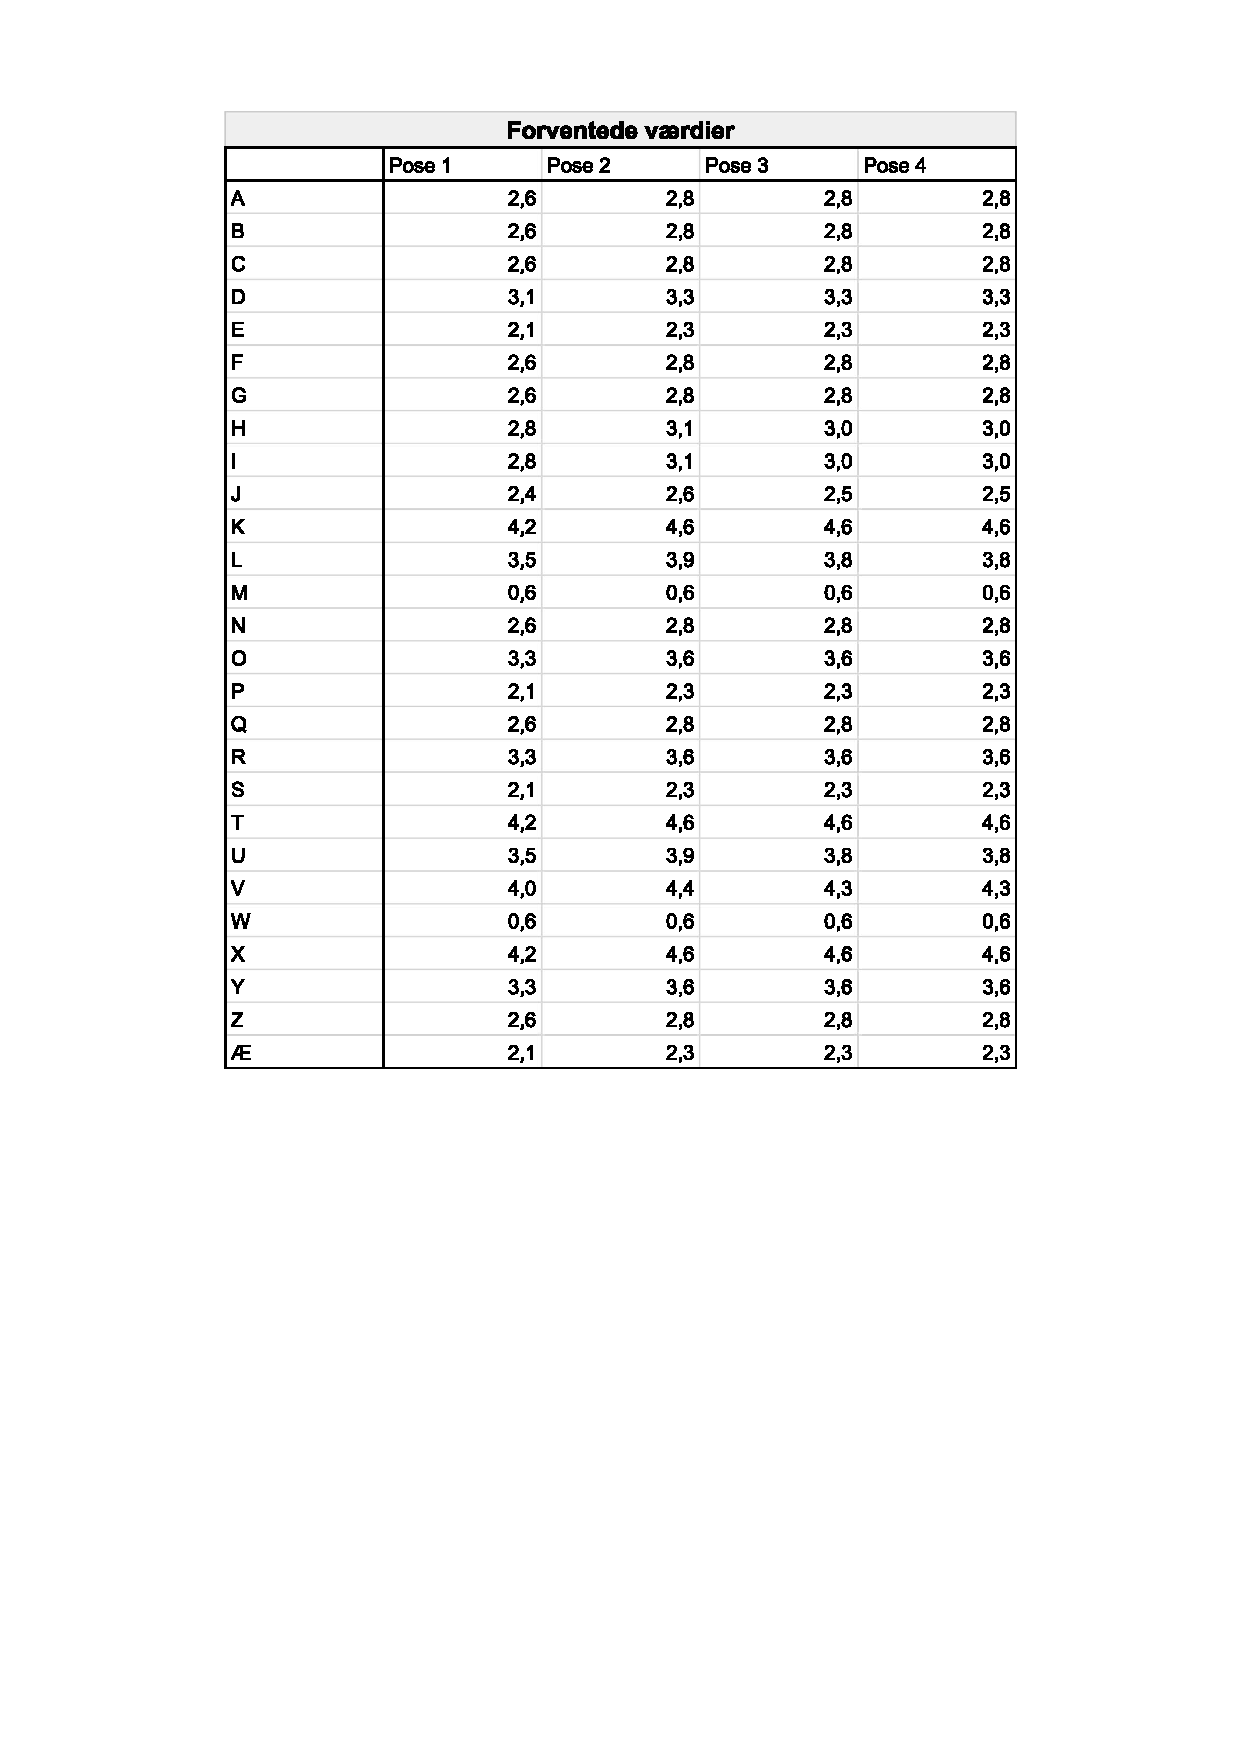
\includegraphics[width=8in]{tabeller/ForventedeVardierUdenInddeling.pdf}
\end{center}

\subsection{Bilag2}\label{bilag2}

\begin{center}
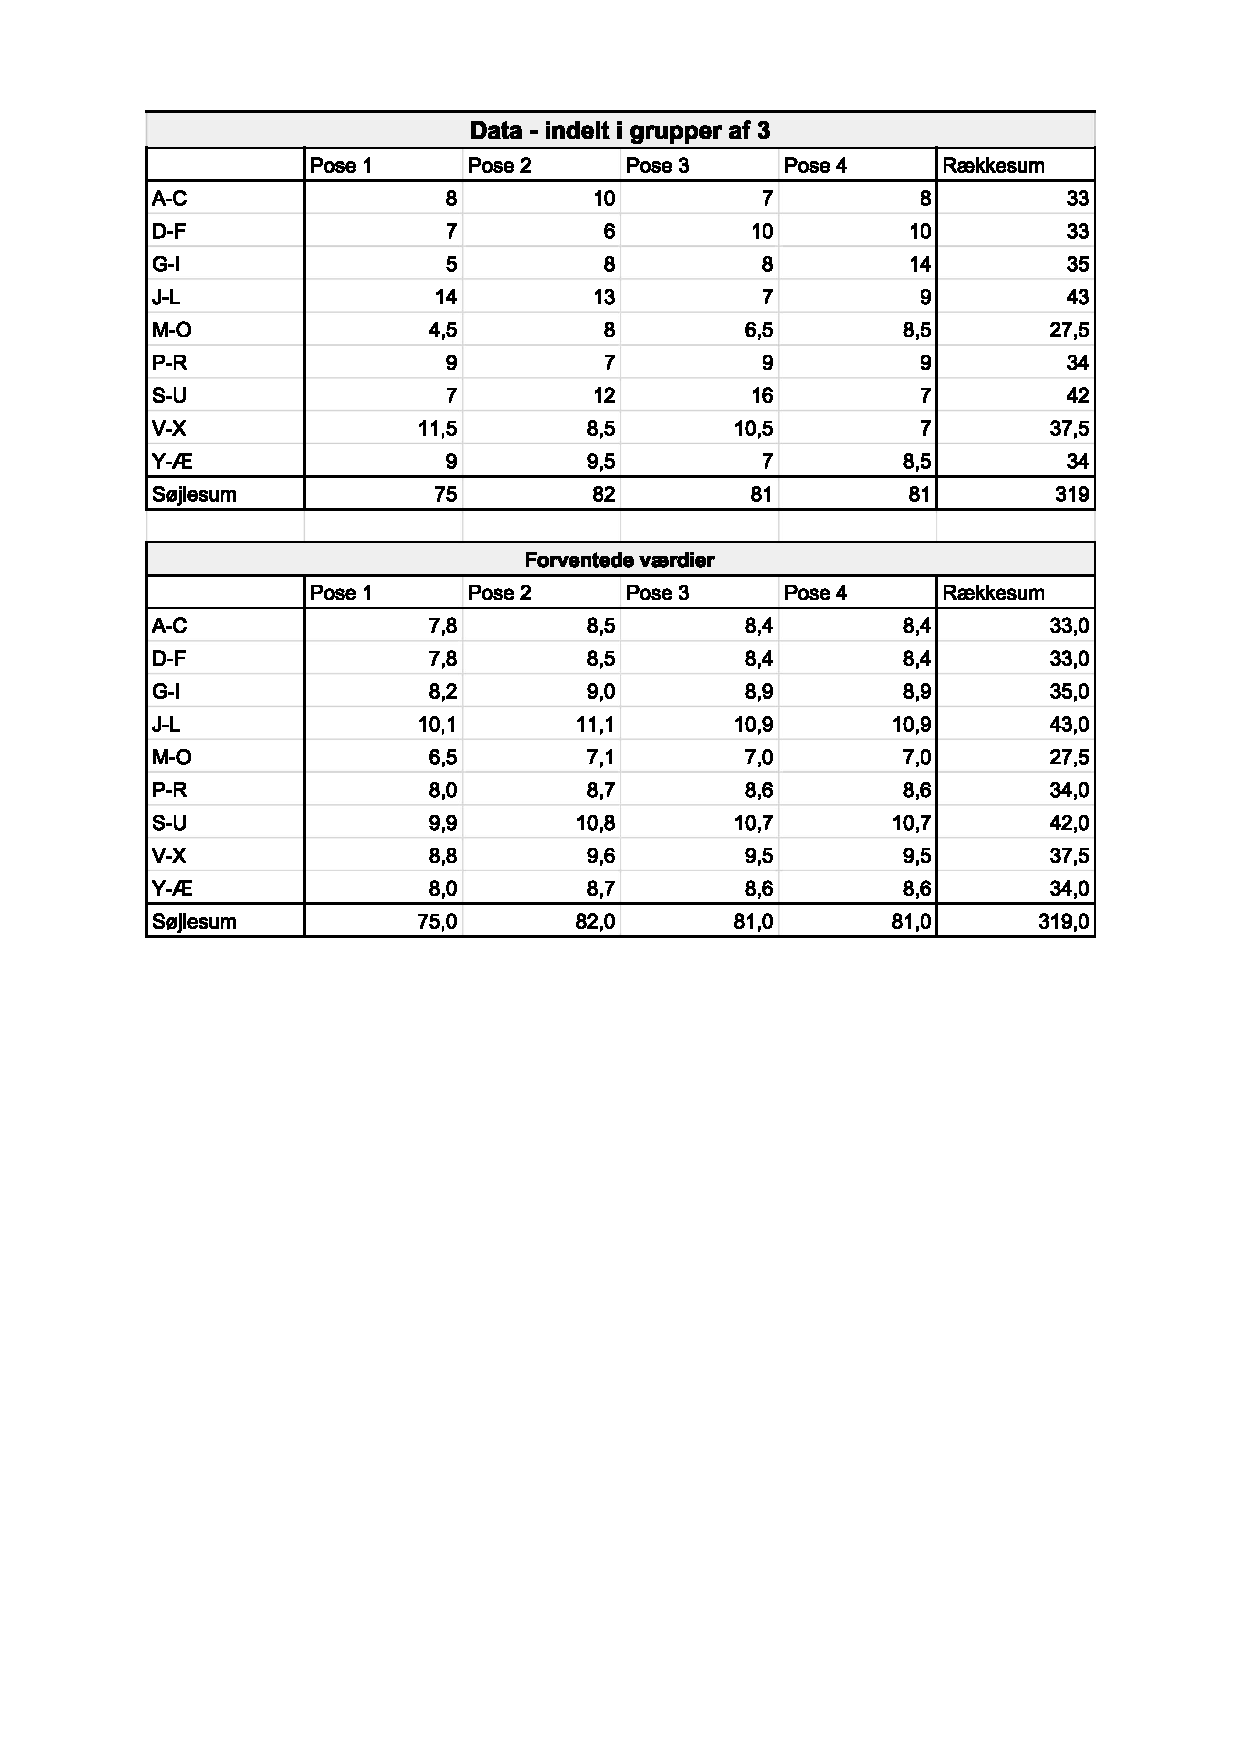
\includegraphics[width=8in]{tabeller/GruperetDataOgForventedeVardier.pdf}
\end{center}


\end{document}
